\documentclass[a4paper,12pt]{article}
\usepackage[margin=18mm]{geometry}
\usepackage{tikz}
\usepackage{amsmath}
\usepackage{xcolor}
\newcommand{\pFourCell}[2]{\makebox[#1em][c]{\ensuremath{#2}}}
\newcommand{\pFourCenterBox}[1]{\begingroup\setbox0=\hbox{$\displaystyle #1$}\dimen0=\ht0\advance\dimen0 by -\dp0\divide\dimen0 by 2\lower\dimen0\box0\endgroup}
\newdimen\pFourFractionRuleThickness
\pFourFractionRuleThickness=0.4pt
\newcommand{\pFourTopAlign}[3]{\raisebox{-#1}[0pt][\dimexpr #1 + #2\relax]{\ensuremath{\displaystyle #3}}}
\newcommand{\pFourBottomAlign}[3]{\raisebox{#2}[\dimexpr #1 + #2\relax][0pt]{\ensuremath{\displaystyle #3}}}
\newcommand{\pFourFractionInner}[2]{\hbox to #1{\hss$\displaystyle #2$\hss}}
\newcommand{\pFourFractionC}[4]{\begingroup\color{#1}\genfrac{}{}{\pFourFractionRuleThickness}{0}{\raisebox{0.14em}{\pFourFractionInner{#2}{{\color{black}#3}}}}{\raisebox{-0.18em}{\pFourFractionInner{#2}{{\color{black}#4}}}}\endgroup}
\newcommand{\pFourFraction}[3]{\genfrac{}{}{\pFourFractionRuleThickness}{0}{\raisebox{0.14em}{\pFourFractionInner{#1}{#2}}}{\raisebox{-0.18em}{\pFourFractionInner{#1}{#3}}}}
\newcommand{\pFourRootC}[2]{\begingroup\setbox0=\hbox{$\displaystyle #2$}\setbox2=\hbox{$\displaystyle \sqrt{\phantom{\copy0}}$}\dimen0=\wd2\advance\dimen0 by -\wd0\hbox{\rlap{\textcolor{#1}{\copy2}}\kern\dimen0\box0}\endgroup}
\newcommand{\pFourRoot}[1]{\pFourRootC{black}{#1}}
\newcommand{\pFourRootDegreeC}[3]{\begingroup\setbox0=\hbox{$\displaystyle #3$}\setbox2=\hbox{$\displaystyle \sqrt[#2]{\phantom{\copy0}}$}\dimen0=\wd2\advance\dimen0 by -\wd0\hbox{\rlap{\textcolor{#1}{\copy2}}\kern\dimen0\box0}\endgroup}
\newcommand{\pFourRootDegree}[2]{\pFourRootDegreeC{black}{#1}{#2}}
\pagestyle{empty}
\begin{document}

\section*{Spaltentreue LaTeX-Ausgabe}
\noindent Gleichung: \texttt{B}\texttt{\textasciicircum{}}\texttt{x}\texttt{=}\texttt{y}\texttt{/}\texttt{a} \hfill Zielvariable: \texttt{x} \hfill Profil: \texttt{standard}

\vspace{8mm}
\begin{center}
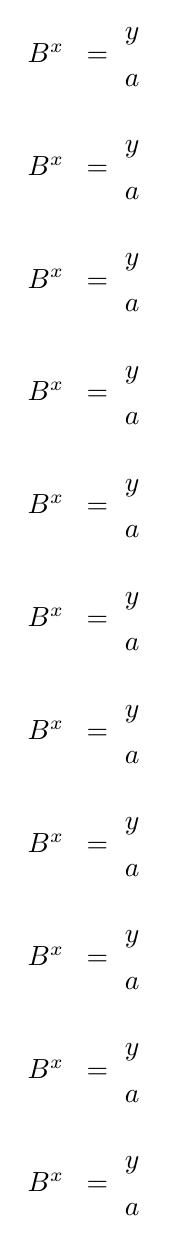
\begin{tikzpicture}[x=1em,y=-1em]
\node[anchor=base, inner sep=0pt] at (4.17,2.75) {$\pFourFraction{0.9em}{\pFourCell{0.9}{y}}{\pFourCell{0.9}{a}}$};
\node[anchor=base, inner sep=0pt] at (1.05,2.75) {$B^{{\scriptstyle x}}$};
\node[anchor=base, inner sep=0pt] at (2.91,2.75) {$\pFourCell{1.62}{=}$};
\node[anchor=base, inner sep=0pt] at (4.17,6.83) {$\pFourFraction{0.9em}{\pFourCell{0.9}{y}}{\pFourCell{0.9}{a}}$};
\node[anchor=base, inner sep=0pt] at (1.05,6.83) {$B^{{\scriptstyle x}}$};
\node[anchor=base, inner sep=0pt] at (2.91,6.83) {$\pFourCell{1.62}{=}$};
\node[anchor=base, inner sep=0pt] at (4.17,10.91) {$\pFourFraction{0.9em}{\pFourCell{0.9}{y}}{\pFourCell{0.9}{a}}$};
\node[anchor=base, inner sep=0pt] at (1.05,10.91) {$B^{{\scriptstyle x}}$};
\node[anchor=base, inner sep=0pt] at (2.91,10.91) {$\pFourCell{1.62}{=}$};
\node[anchor=base, inner sep=0pt] at (4.17,14.99) {$\pFourFraction{0.9em}{\pFourCell{0.9}{y}}{\pFourCell{0.9}{a}}$};
\node[anchor=base, inner sep=0pt] at (1.05,14.99) {$B^{{\scriptstyle x}}$};
\node[anchor=base, inner sep=0pt] at (2.91,14.99) {$\pFourCell{1.62}{=}$};
\node[anchor=base, inner sep=0pt] at (4.17,19.07) {$\pFourFraction{0.9em}{\pFourCell{0.9}{y}}{\pFourCell{0.9}{a}}$};
\node[anchor=base, inner sep=0pt] at (1.05,19.07) {$B^{{\scriptstyle x}}$};
\node[anchor=base, inner sep=0pt] at (2.91,19.07) {$\pFourCell{1.62}{=}$};
\node[anchor=base, inner sep=0pt] at (4.17,23.15) {$\pFourFraction{0.9em}{\pFourCell{0.9}{y}}{\pFourCell{0.9}{a}}$};
\node[anchor=base, inner sep=0pt] at (1.05,23.15) {$B^{{\scriptstyle x}}$};
\node[anchor=base, inner sep=0pt] at (2.91,23.15) {$\pFourCell{1.62}{=}$};
\node[anchor=base, inner sep=0pt] at (4.17,27.23) {$\pFourFraction{0.9em}{\pFourCell{0.9}{y}}{\pFourCell{0.9}{a}}$};
\node[anchor=base, inner sep=0pt] at (1.05,27.23) {$B^{{\scriptstyle x}}$};
\node[anchor=base, inner sep=0pt] at (2.91,27.23) {$\pFourCell{1.62}{=}$};
\node[anchor=base, inner sep=0pt] at (4.17,31.31) {$\pFourFraction{0.9em}{\pFourCell{0.9}{y}}{\pFourCell{0.9}{a}}$};
\node[anchor=base, inner sep=0pt] at (1.05,31.31) {$B^{{\scriptstyle x}}$};
\node[anchor=base, inner sep=0pt] at (2.91,31.31) {$\pFourCell{1.62}{=}$};
\node[anchor=base, inner sep=0pt] at (4.17,35.39) {$\pFourFraction{0.9em}{\pFourCell{0.9}{y}}{\pFourCell{0.9}{a}}$};
\node[anchor=base, inner sep=0pt] at (1.05,35.39) {$B^{{\scriptstyle x}}$};
\node[anchor=base, inner sep=0pt] at (2.91,35.39) {$\pFourCell{1.62}{=}$};
\node[anchor=base, inner sep=0pt] at (4.17,39.47) {$\pFourFraction{0.9em}{\pFourCell{0.9}{y}}{\pFourCell{0.9}{a}}$};
\node[anchor=base, inner sep=0pt] at (1.05,39.47) {$B^{{\scriptstyle x}}$};
\node[anchor=base, inner sep=0pt] at (2.91,39.47) {$\pFourCell{1.62}{=}$};
\node[anchor=base, inner sep=0pt] at (4.17,43.55) {$\pFourFraction{0.9em}{\pFourCell{0.9}{y}}{\pFourCell{0.9}{a}}$};
\node[anchor=base, inner sep=0pt] at (1.05,43.55) {$B^{{\scriptstyle x}}$};
\node[anchor=base, inner sep=0pt] at (2.91,43.55) {$\pFourCell{1.62}{=}$};
\end{tikzpicture}
\end{center}


\newpage
\section*{Spaltentreue LaTeX-Ausgabe mit Spaltengrenzen}
\vspace{6mm}
\begin{center}
\begin{tikzpicture}[x=1em,y=-1em]
\node[font={\scriptsize}, text=gray!65, anchor=west] at (0,-0.75) {Spaltengrenzen: blau; Spaltenmitten: grau gepunktet; lokale Bruch-/Span-Achsen: rot};
\draw[blue!22, line width=0.28pt] (0,0.35) -- (0,45.83);
\draw[blue!22, line width=0.28pt] (2.1,0.35) -- (2.1,45.83);
\draw[blue!22, line width=0.28pt] (3.72,0.35) -- (3.72,45.83);
\draw[blue!22, line width=0.28pt] (4.62,0.35) -- (4.62,45.83);
\draw[gray!35, dotted] (1.05,0.35) -- (1.05,45.83);
\node[font={\ttfamily\scriptsize}, text=gray!70, anchor=base] at (1.05,0) {0};
\draw[gray!35, dotted] (2.91,0.35) -- (2.91,45.83);
\node[font={\ttfamily\scriptsize}, text=gray!70, anchor=base] at (2.91,0) {1};
\draw[gray!35, dotted] (4.17,0.35) -- (4.17,45.83);
\node[font={\ttfamily\scriptsize}, text=gray!70, anchor=base] at (4.17,0) {2};
\draw[red!30, opacity=0.32, line width=0.35pt] (4.17,1) -- (4.17,4.13);
\node[anchor=base, inner sep=0pt] at (4.17,2.75) {$\pFourFraction{0.9em}{\pFourCell{0.9}{y}}{\pFourCell{0.9}{a}}$};
\node[anchor=base, inner sep=0pt] at (1.05,2.75) {$B^{{\scriptstyle x}}$};
\node[anchor=base, inner sep=0pt] at (2.91,2.75) {$\pFourCell{1.62}{=}$};
\draw[red!30, opacity=0.32, line width=0.35pt] (4.17,5.08) -- (4.17,8.21);
\node[anchor=base, inner sep=0pt] at (4.17,6.83) {$\pFourFraction{0.9em}{\pFourCell{0.9}{y}}{\pFourCell{0.9}{a}}$};
\node[anchor=base, inner sep=0pt] at (1.05,6.83) {$B^{{\scriptstyle x}}$};
\node[anchor=base, inner sep=0pt] at (2.91,6.83) {$\pFourCell{1.62}{=}$};
\draw[red!30, opacity=0.32, line width=0.35pt] (4.17,9.16) -- (4.17,12.29);
\node[anchor=base, inner sep=0pt] at (4.17,10.91) {$\pFourFraction{0.9em}{\pFourCell{0.9}{y}}{\pFourCell{0.9}{a}}$};
\node[anchor=base, inner sep=0pt] at (1.05,10.91) {$B^{{\scriptstyle x}}$};
\node[anchor=base, inner sep=0pt] at (2.91,10.91) {$\pFourCell{1.62}{=}$};
\draw[red!30, opacity=0.32, line width=0.35pt] (4.17,13.24) -- (4.17,16.37);
\node[anchor=base, inner sep=0pt] at (4.17,14.99) {$\pFourFraction{0.9em}{\pFourCell{0.9}{y}}{\pFourCell{0.9}{a}}$};
\node[anchor=base, inner sep=0pt] at (1.05,14.99) {$B^{{\scriptstyle x}}$};
\node[anchor=base, inner sep=0pt] at (2.91,14.99) {$\pFourCell{1.62}{=}$};
\draw[red!30, opacity=0.32, line width=0.35pt] (4.17,17.32) -- (4.17,20.45);
\node[anchor=base, inner sep=0pt] at (4.17,19.07) {$\pFourFraction{0.9em}{\pFourCell{0.9}{y}}{\pFourCell{0.9}{a}}$};
\node[anchor=base, inner sep=0pt] at (1.05,19.07) {$B^{{\scriptstyle x}}$};
\node[anchor=base, inner sep=0pt] at (2.91,19.07) {$\pFourCell{1.62}{=}$};
\draw[red!30, opacity=0.32, line width=0.35pt] (4.17,21.4) -- (4.17,24.53);
\node[anchor=base, inner sep=0pt] at (4.17,23.15) {$\pFourFraction{0.9em}{\pFourCell{0.9}{y}}{\pFourCell{0.9}{a}}$};
\node[anchor=base, inner sep=0pt] at (1.05,23.15) {$B^{{\scriptstyle x}}$};
\node[anchor=base, inner sep=0pt] at (2.91,23.15) {$\pFourCell{1.62}{=}$};
\draw[red!30, opacity=0.32, line width=0.35pt] (4.17,25.48) -- (4.17,28.61);
\node[anchor=base, inner sep=0pt] at (4.17,27.23) {$\pFourFraction{0.9em}{\pFourCell{0.9}{y}}{\pFourCell{0.9}{a}}$};
\node[anchor=base, inner sep=0pt] at (1.05,27.23) {$B^{{\scriptstyle x}}$};
\node[anchor=base, inner sep=0pt] at (2.91,27.23) {$\pFourCell{1.62}{=}$};
\draw[red!30, opacity=0.32, line width=0.35pt] (4.17,29.56) -- (4.17,32.69);
\node[anchor=base, inner sep=0pt] at (4.17,31.31) {$\pFourFraction{0.9em}{\pFourCell{0.9}{y}}{\pFourCell{0.9}{a}}$};
\node[anchor=base, inner sep=0pt] at (1.05,31.31) {$B^{{\scriptstyle x}}$};
\node[anchor=base, inner sep=0pt] at (2.91,31.31) {$\pFourCell{1.62}{=}$};
\draw[red!30, opacity=0.32, line width=0.35pt] (4.17,33.64) -- (4.17,36.77);
\node[anchor=base, inner sep=0pt] at (4.17,35.39) {$\pFourFraction{0.9em}{\pFourCell{0.9}{y}}{\pFourCell{0.9}{a}}$};
\node[anchor=base, inner sep=0pt] at (1.05,35.39) {$B^{{\scriptstyle x}}$};
\node[anchor=base, inner sep=0pt] at (2.91,35.39) {$\pFourCell{1.62}{=}$};
\draw[red!30, opacity=0.32, line width=0.35pt] (4.17,37.72) -- (4.17,40.85);
\node[anchor=base, inner sep=0pt] at (4.17,39.47) {$\pFourFraction{0.9em}{\pFourCell{0.9}{y}}{\pFourCell{0.9}{a}}$};
\node[anchor=base, inner sep=0pt] at (1.05,39.47) {$B^{{\scriptstyle x}}$};
\node[anchor=base, inner sep=0pt] at (2.91,39.47) {$\pFourCell{1.62}{=}$};
\draw[red!30, opacity=0.32, line width=0.35pt] (4.17,41.8) -- (4.17,44.93);
\node[anchor=base, inner sep=0pt] at (4.17,43.55) {$\pFourFraction{0.9em}{\pFourCell{0.9}{y}}{\pFourCell{0.9}{a}}$};
\node[anchor=base, inner sep=0pt] at (1.05,43.55) {$B^{{\scriptstyle x}}$};
\node[anchor=base, inner sep=0pt] at (2.91,43.55) {$\pFourCell{1.62}{=}$};
\end{tikzpicture}
\end{center}
\end{document}
